\documentclass[TIDYMASTER.tex]{subfiles} 
\begin{document} 


	%===============================================%
	\begin{frame}
	
		\begin{figure}
			\centering
		
\includegraphics[width=0.65\linewidth]{images/TidyRLogo}
		\end{figure}
		\[\mbox{Coding Grace - Workshop 2016}\]
	\end{frame}
%=================================================== %		
%=============================================================================== %
\begin{frame}
	\frametitle{Tidy Data with \texttt{R}}
	\large
	\begin{framed}
		“Tidy datasets are all alike but every messy dataset is messy in its own way.” – Hadley Wickham
	\end{framed}
	
	\begin{framed}
		\begin{quote}
			Data science, at its heart, is a computer programming exercise. Data scientists use computers to store, transform, visualize, and model their data. As a result, every data science project begins with the same task: you must prepare your data to use it with a computer.
		\end{quote} 
	\end{framed}
\end{frame}
	%===============================================%
	\begin{frame}
		\vspace{-0.5cm}
		\LARGE		\begin{figure}
			\centering
			
\includegraphics[width=0.35\linewidth]{images/dplyr-hexbin-logo}
			
\includegraphics[width=0.35\linewidth]{images/TidyRLogo}
		
\includegraphics[width=0.35\linewidth]{images/magrittr}
\end{figure}
		\begin{itemize}
			\item \textbf{dplyr} - data manipulation
			
			
			\item \textbf{magrittr} - pipe operator
		\end{itemize}
		
	\end{frame}

	%===================================================================== %
	\begin{frame}
		\frametitle{Tidy Data}
		\Large
		\vspace{-1.5cm}
		\noindent{Abstract from \textbf{dplyr} talk}
		\begin{itemize}
			
			\item To make the most of dplyr, Hadley Wickham recommends that you familiarise yourself with the \textbf{principles of tidy data}. 
			\item This will help you get your data into a form that works well with \textbf{dplyr}, \textbf{ggplot2} and \texttt{R}'s many modelling functions.
		\end{itemize}
	\end{frame}
%========================================= %	
\begin{frame}
	\frametitle{Tidy Data With \texttt{R}}
	\Large
	\vspace{-1cm}
	\begin{itemize}
		\item \textbf{tidyr} is a reframing of reshape2 designed to accompany the tidy data framework, and to work hand-in-hand with \textbf{magrittr} and \textbf{dplyr} to build a solid pipeline for data analysis. \\ \textit{(from Hadley Wickham's abstract)}
	\end{itemize}
	
	
\end{frame}
%========================================= %
\begin{frame}[fragile]
	\frametitle{Principles of Tidy Data}
	\Large
	\begin{itemize}
		\item 	Tidy data was popularized by Hadley Wickham, and it serves as the basis for many R packages and functions. 
		\item You can learn more about tidy data by reading \textbf{Tidy Data} a paper written by Hadley Wickham and published in the Journal of Statistical Software. 
		\item Tidy Data is available online at \begin{verbatim}
		www.jstatsoft.org/v59/i10/paper.
		\end{verbatim}
	\end{itemize}
\end{frame}	
	%====================================================================== %
	\begin{frame}[fragile]
		\textbf{Tidy Data}
		\begin{framed}
			\noindent Three Principles from Hadley Wickham's paper
			\begin{itemize}
				\item[1.] Each variable forms a column, 
				\item[2.] Each observation forms a row, 
				\item[3.] Each table/file stores data about one kind of observation.
			\end{itemize}
		\end{framed}
		\noindent \textbf{Remark:} \\  The paper ``\textit{\textbf{Tidy Data}}" by Hadley Wickham (RStudio) can be downloaded from 
		\begin{verbatim}
		http://vita.had.co.nz/papers/tidy-data.pdf
		\end{verbatim}
	\end{frame}
%========================================== %
\begin{frame}[fragile]
	\frametitle{Tidy Data with \texttt{R}}
	\Large

	
	\texttt{R} follows a set of conventions that makes one layout of tabular data much easier to work with than others.
	
	\begin{itemize}
				\item \textbf{Each column is a variable:} Each variable in the data set is placed in its \textbf{own} column
					\item \textbf{Each row is an observation:}
		Each observation is placed in its \textbf{own} row
		\item Each value is placed in its own cell

		
	\end{itemize}
	Data that satisfies these rules is known as \textbf{tidy data}.
 %Notice that table1 is tidy data.
\end{frame}
%=============================================================================== %
\begin{frame}[fragile]
	\frametitle{Tidy Data with \texttt{R}}
	\Large

	\noindent \textbf{Dataframes} (if you are not familiar)\\
	\begin{itemize}
\item A data frame is a list of vectors that R displays as a table. 
\item When your data is tidy, the values of each variable fall in their own column vector.

	\end{itemize}
	\begin{figure}
\centering
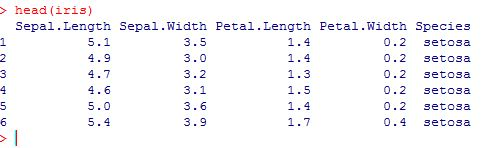
\includegraphics[width=0.7\linewidth]{headiris}

\end{figure}

	\end{frame}
	%=================================================================== %
\begin{frame}
\begin{figure}
\centering
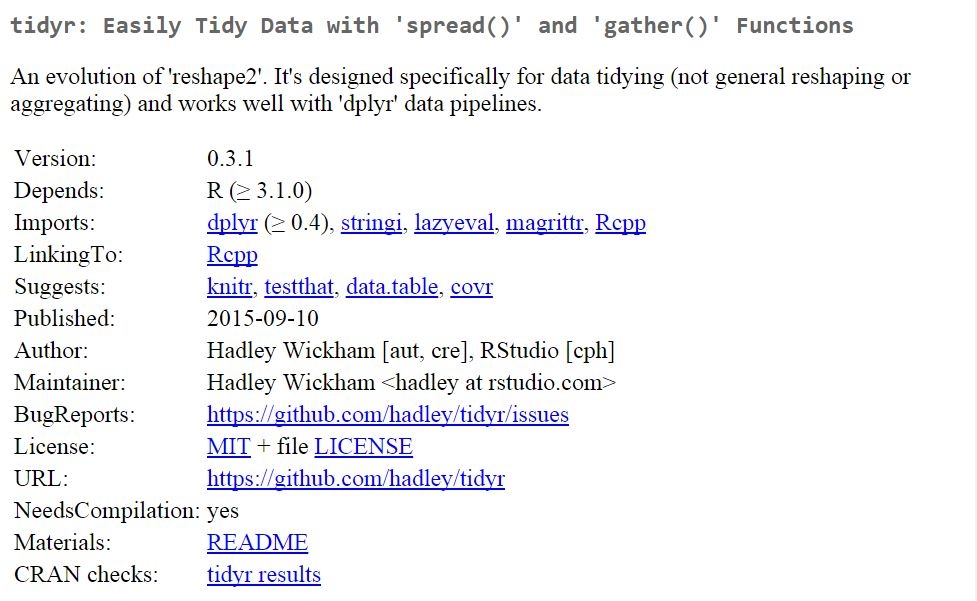
\includegraphics[width=1.1\linewidth]{CRAN-TidyR}
\end{figure}
\end{frame}	
%=====================================================%
\begin{frame}
\frametitle{\texttt{tidyR} }
\Large
\vspace{-0.7cm}
\textit{Abstract for tidyr}
\begin{itemize}
\item tidyr is new package that makes it easy to ``tidy” your data. 
\item Tidy data is data that’s easy to work with: it’s easy to munge (with \textbf{dplyr}), 
visualise (with \textbf{ggplot2} or \textbf{ggvis}) and model (with \texttt{R}'s hundreds of modelling packages). 
\end{itemize}
\end{frame}

%=====================================================%
%\begin{frame}
%\frametitle{\texttt{tidyR} }
%Arranging your data in this way makes it easier to work with because you have a consistent way of referring to variables (as column names) and observations (as row indices). When use tidy data and tidy tools, you spend less time worrying about how to feed the output from one function into the input of another, and more time answering your questions about the data.
%\end{frame}

%=====================================================%
\begin{frame}[fragile]
	\frametitle{\texttt{tidyR} }
\Large
\noindent \textbf{tidyr's verbs}
\begin{itemize}
%\item To tidy messy data, you first identify the variables in your dataset.
%\item Then you can use the tools provided by tidyr to move them into columns. 
\item \textbf{tidyr} provides four main functions for tidying your messy data: \texttt{gather()}, \texttt{separate()}, \texttt{spread()} and \texttt{unite()}.
\end{itemize}
{
	\Large
\begin{framed}
\begin{verbatim}
gather()
spread()
separate()
unite()
\end{verbatim}
\end{framed}
}
\end{frame}
\end{document}




























